\begin{frame}{Applikation}
	\begin{center}
		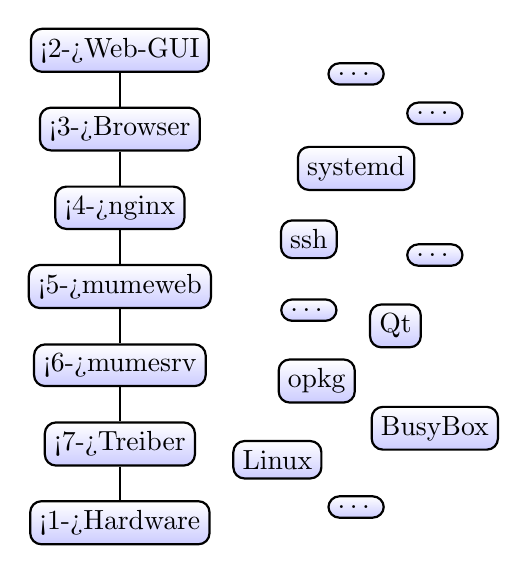
\begin{tikzpicture}[thick]
			\tikzstyle{every node}=[shape=rectangle, rounded corners,
				draw, align=center, top color=white, bottom color=blue!20]
			\node at (0,0) (hw) {{\visible<1->{Hardware}}};
			\node at (0,1) (driver) {{\visible<7->{Treiber}}};
			\node at (0,2) (srv) {{\visible<6->{mumesrv}}};
			\node at (0,3) (web) {{\visible<5->{mumeweb}}};
			\node at (0,4) (server) {{\visible<4->{nginx}}};
			\node at (0,5) (browser) {{\visible<3->{Browser}}};
			\node at (0,6) (gui) {{\visible<2->{Web-GUI}}};
			
			\visible<8-> {
				\node at (2,0.8) {Linux};
				\node at (4,1.2) {BusyBox};
				\node at (2.5,1.8) {opkg};
				\node at (3.5,2.5) {Qt};
				\node at (2.4,3.6) {ssh};
				\node at (3,4.5) {systemd};
			}
			
			\visible<9-> {
				\node at (2.4,2.7) {\ldots};
				\node at (3,0.2) {\ldots};
				\node at (4,3.4) {\ldots};
				\node at (4,5.2) {\ldots};
				\node at (3,5.7) {\ldots};
			}
			
			\draw (hw) -- (driver);
			\draw (driver) -- (srv);
			\draw (srv) -- (web);
			\draw (web) -- (server);
			\draw (server) -- (browser);
			\draw (browser) -- (gui);
		\end{tikzpicture}
	\end{center}
\end{frame}

\begin{frame}{Hardware}
	\begin{multicols}{2}
		\begin{center}
			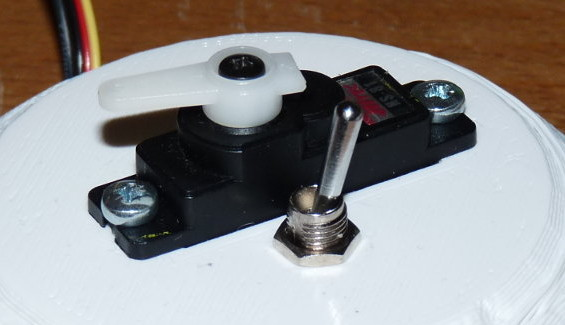
\includegraphics[height=3cm]{res/mume_urs.jpg}
		\end{center}
		\pause
		\begin{center}
			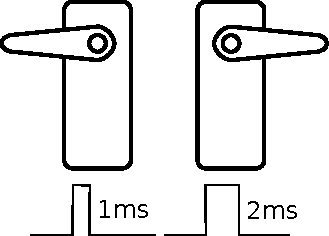
\includegraphics[height=3cm]{res/servo_pwm.pdf}
		\end{center}
	\end{multicols}
\end{frame}

\begin{frame}[fragile]{mume Device Tree}
	\begin{multicols}{2}
		\begin{lstlisting}[frame=,numbers=none,language=]
mume {
  compatible = "urs,mume";
  status = "okay";

  gpio = <&gpio1 28 GPIO_ACTIVE_LOW>;
  pwms = <&ehrpwm1 0 10000000 0>;

  pinctrl-names = "default";
  pinctrl-0 = <&mume_pins>;
};

mume_pins: mume_pins {
  pinctrl-single,pins = <
    0x78 (MUX_MODE7 | PIN_INPUT_PULLUP)
    0x48 (MUX_MODE6 | PIN_OUTPUT)
  >;
};
		\end{lstlisting}
\pagebreak
		\begin{flushright}
		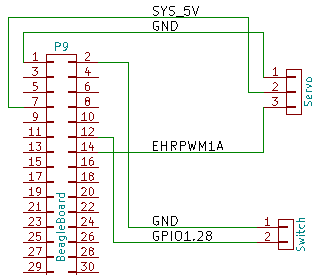
\includegraphics[width=4.3cm]{res/mume_schematic.pdf}
		\end{flushright}
	\end{multicols}
\end{frame}

\begin{frame}{Hardware ansteuern}
	\begin{multicols}{2}
		\begin{center}
			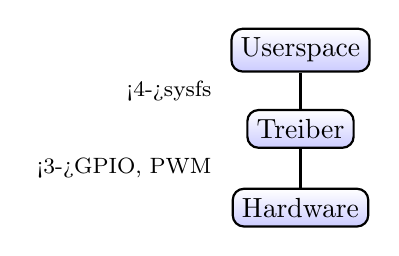
\begin{tikzpicture}[thick,
				every node/.style = {shape=rectangle, rounded corners,
					draw, align=center,
					top color=white, bottom color=blue!20}]]

				\node (userspace) {Userspace};
				\node[below of=userspace] (driver) {Treiber};
				\node[below of=driver] (hardware) {Hardware};

				\tikzstyle{every node}=[midway,left=10mm,font=\footnotesize]
				\draw (driver) -- (hardware) node {{\visible<3->{GPIO, PWM}}};
				\draw (userspace) -- (driver) node {{\visible<4->{sysfs}}};
			\end{tikzpicture}
			\visible<2->{
				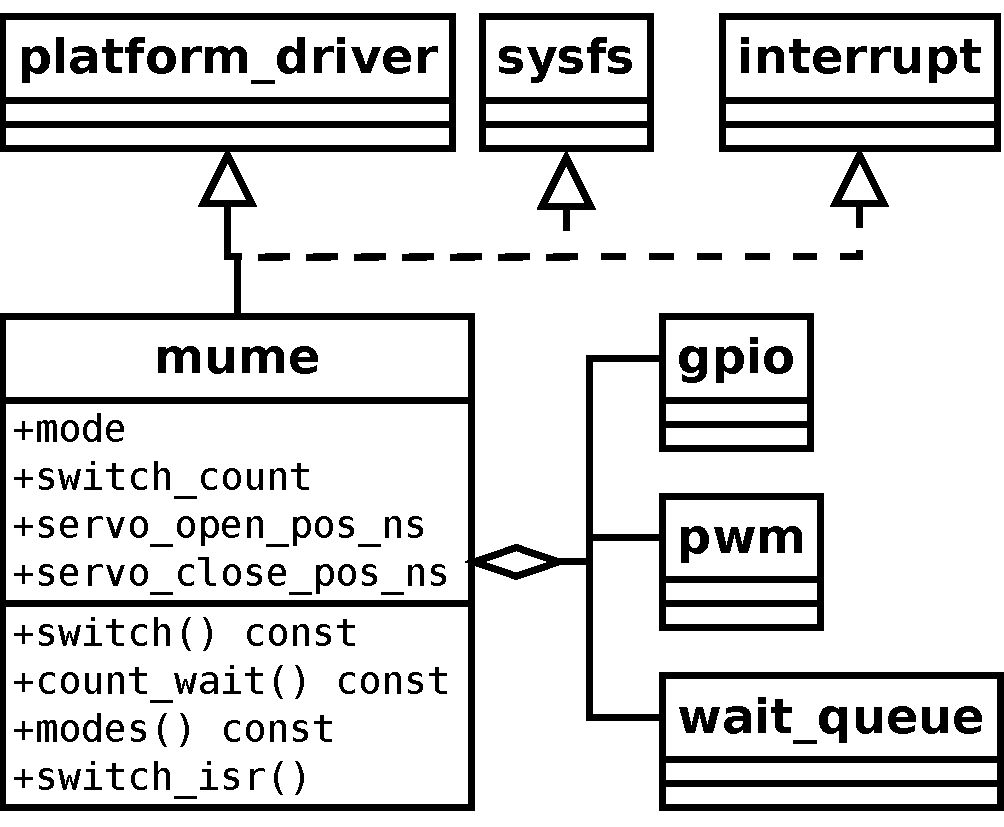
\includegraphics[width=0.5\textwidth]{res/mumedriver}
			}
		\end{center}
	\end{multicols}
	\only<handout>{
		\begin{itemize}
			\item wie können wir die Hardware ansteuern?
			\item[$\rightarrow$] Linux Treiber, Frameworks, Infrastructure:
			\begin{itemize}
				\item Framework für Treiber
				\item Infrastrukur um auf Subsysteme zuzugreifen
			\end{itemize}
		\end{itemize}
	}
\end{frame}

\begin{frame}{vom Treiber zum Webserver}
	\begin{center}
		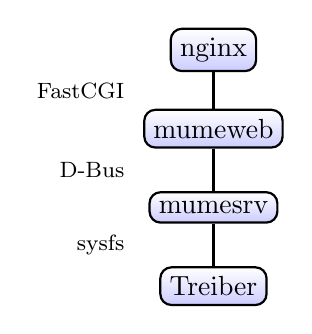
\begin{tikzpicture}[thick]
			\tikzstyle{every node}=[shape=rectangle, rounded corners,
				draw, align=center, top color=white, bottom color=blue!20]

			\node at (0,1) (driver) {Treiber};
			\node at (0,4) (server) {nginx};
			
			\visible<2->{
				\node at (0,2) (srv) {mumesrv};
			}
			
			\visible<3->{
				\node at (0,3) (web) {mumeweb};
			}

			\tikzstyle{every node}=[midway,left=10mm,font=\footnotesize]
			\visible<2->{
				\draw (driver) -- (srv) node {sysfs};
			}
			\visible<3->{
				\draw (web) -- (server) node {FastCGI};
			}
			\visible<4->{
				\draw (srv) -- (web) node {D-Bus};
			}
			
		\end{tikzpicture}
	\end{center}
\end{frame}
\note{
	\begin{itemize}
		\item mumeweb
		\begin{itemize}
			\item FastCGI / XML Interface
			\item (Session Handling)
		\end{itemize}
		\item mumesrv
		\begin{itemize}
			\item Persistenz
			\item D-Bus Interface
		\end{itemize}
	\end{itemize}
}

\begin{frame}[fragile]{Starten der Services}
	\begin{itemize}
		\item systemd / unit file
	\end{itemize}
	\begin{lstlisting}[frame=single,basicstyle=\small\ttfamily,escapeinside={|}{|},language=]
[Unit]
Description=Mume D-Bus Service
After=dbus.target
Wants=dbus.target

[Service]
ExecStart=/usr/bin/mumesrv /sys/|\ldots|/mume/

[Install]
WantedBy=multi-user.target
	\end{lstlisting}
\end{frame}

\begin{frame}[fragile]{mumesrv Rezept}
	\begin{lstlisting}[frame=single,language=bitbake]
SECTION = "app"
DESCRIPTION = "MUME D-Bus interface to hardware"
LICENSE = "GPLv3+"
LIC_FILES_CHKSUM = "file://COPYING;md5=9eef91148a9b14ec7f9df333daebc746"

inherit qmake5

DEPENDS += "qtbase"
RDEPENDS_${PN} += "qtbase dbus"

SRCREV = "3cbe61c102d9574ccd039b112704f0a42a2112f8"

SRC_URI = " \
	git://github.com/ursfassler/mumesrv.git;protocol=https;branch=master \
	file://dbus.conf \
"

S = "${WORKDIR}/git"
QMAKE_PROFILES = "${S}/application/application.pro"
@\ldots@
	\end{lstlisting}
\end{frame}

\begin{frame}[fragile]{Produktiv Image}
	\begin{lstlisting}[title=mume-image.bb,frame=single,language=bitbake]
LICENSE = "MIT"

inherit core-image

IMAGE_INSTALL = " \
  packagegroup-core-boot \
  packagegroup-core-ssh-openssh \
  packagegroup-mume-common \
  \
  mumesrv-start \
  mumeweb-start \
"

IMAGE_FEATURES += " \
  package-management \
"
	\end{lstlisting}
	\pause
	\begin{lstlisting}[frame=single,language=bash, basicstyle=\small\ttfamily]
$ bitbake mume-image
	\end{lstlisting}
\end{frame}
\note{
	\begin{itemize}
		\item Wie können wir die Firmware verteilen?
		\item[$\rightarrow$] Yocto
		\begin{itemize}
			\item Rezepte für Services
			\item anpassen bestehender Rezepte (nginx, qt, \ldots)
			\item Rezept für Image
		\end{itemize}
		\item bitbake image
	\end{itemize}
}

%\begin{frame}{Was passiert bei einem Tastendruck in der Web-Applikation}
%	Geht runter:
%	\begin{itemize}
%		\item SVG, Javascript
%		\item XML/HTTP
%		\item FastCGI
%		\item MumeWeb
%		\item D-Bus
%		\item MumeSrv
%		\item SysFS
%		\item Kernel
%		\item MUME-Treiber
%		\item PWM
%		\item Servo bewegt sich!
%	\end{itemize}
%\end{frame}
